\chapter{实验结果分析}
\section{算法总体性能测试}

首先是算法整体性能测试,本次测试所用的矩阵主要来自于\cite{park2014sparsifying}和\cite{liuSyncFree2016}这两片文章中所用到的矩阵,这些矩阵都可以从MatrixMarket和弗罗里达大学稀疏矩阵集合中下载。本次测试我所使用的矩阵如表\ref{MatrixSuite}所示。表中最后一列并行性的定义为并行性=最大level数$ \div $算法的行数,可以理解为平均每个level有多少的任务,其中并行性最好的是矩阵nlpkkt160,只有两个level,理论并行性最差的是hollywood-2009和crankseg\_1。


\begin{table}[htbp]
    \resizebox{\textwidth}{!}{%
    \begin{tabular}{|l|r|r|r|r|}
    \hline
    矩阵名称           & 行或列数量      & 非零元个数       & 最大level数 & 并行性 \\ \hline
    nlpkkt160      & 8,345,600  & 229,518,112 & 2        & 4,172,800   \\
    road\_central   & 14,081,816 & 33,866,826  & 59       & 238,675     \\
    road\_usa       & 23,947,347 & 57,708,624  & 77       & 311,004     \\
    webbase-1M     & 1,000,005  & 3,105,536   & 514      & 1,946       \\
    wiki-Talk      & 2,394,385  & 5,021,410   & 522      & 4,587       \\
    chipcool0      & 20,082     & 281,150     & 534      & 37          \\
    crankseg\_1     & 52,804     & 10,614,210  & 4056     & 13          \\ \hline
    \end{tabular}%
    }
    \caption{性能测试所用矩阵}
    \label{MatrixSuite}
\end{table}

这里我对比了不同平台的SpTRSV的算法性能,其中intel平台选用的是MKL11.3版本,CPU为双路志强E5-2695 v3。ARM平台采用鲲鹏920处理器。在GPU平台采用了sync-free的SpTRSV算法,所用硬件为TiTanX,结果如图\ref{SpTRSVMulti-paltform}。

在图\ref{SpTRSVMulti-paltform}中,我分贝测试了6个矩阵,通过5个柱状图的形式,以GFlops为单位显示了算法的性能,GLflops计算方法为$(2 \times NNZL)  \div totoal\_time$。$totoal\_time = preprocess\_time + calculate\_time$。
NNZL表示下三角矩阵非零元的个数,为双精度浮点类型,所以前面乘2。


对于可以看出,由于使用了并行性较好的矩阵如nlpkkt160,road\_central和road\_usa算法都取得了相比于串性算法3倍以上的加速比。而对于那些并行性较差的矩阵如wiki-Talk以及chipcool0算法level数量较多,能够获得加速比较差,但是仍然能够获得一定的加速。

\begin{figure}[htbp]
    \centering
    \subfigure{
    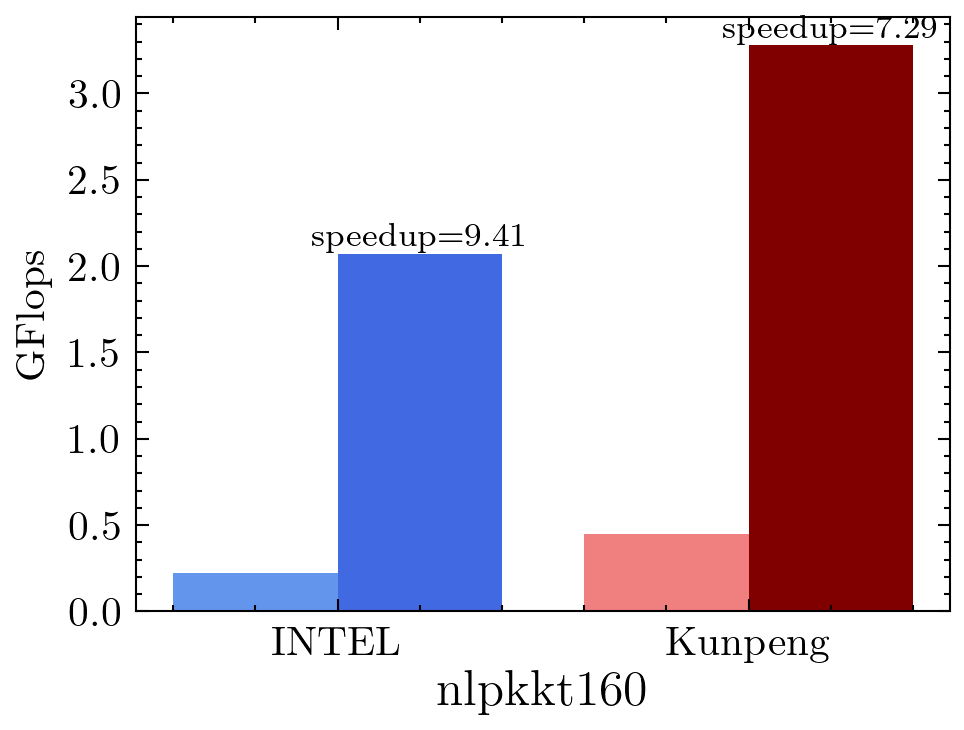
\includegraphics[width=6.5cm]{result0.png}
    }
    \quad
    \subfigure{
    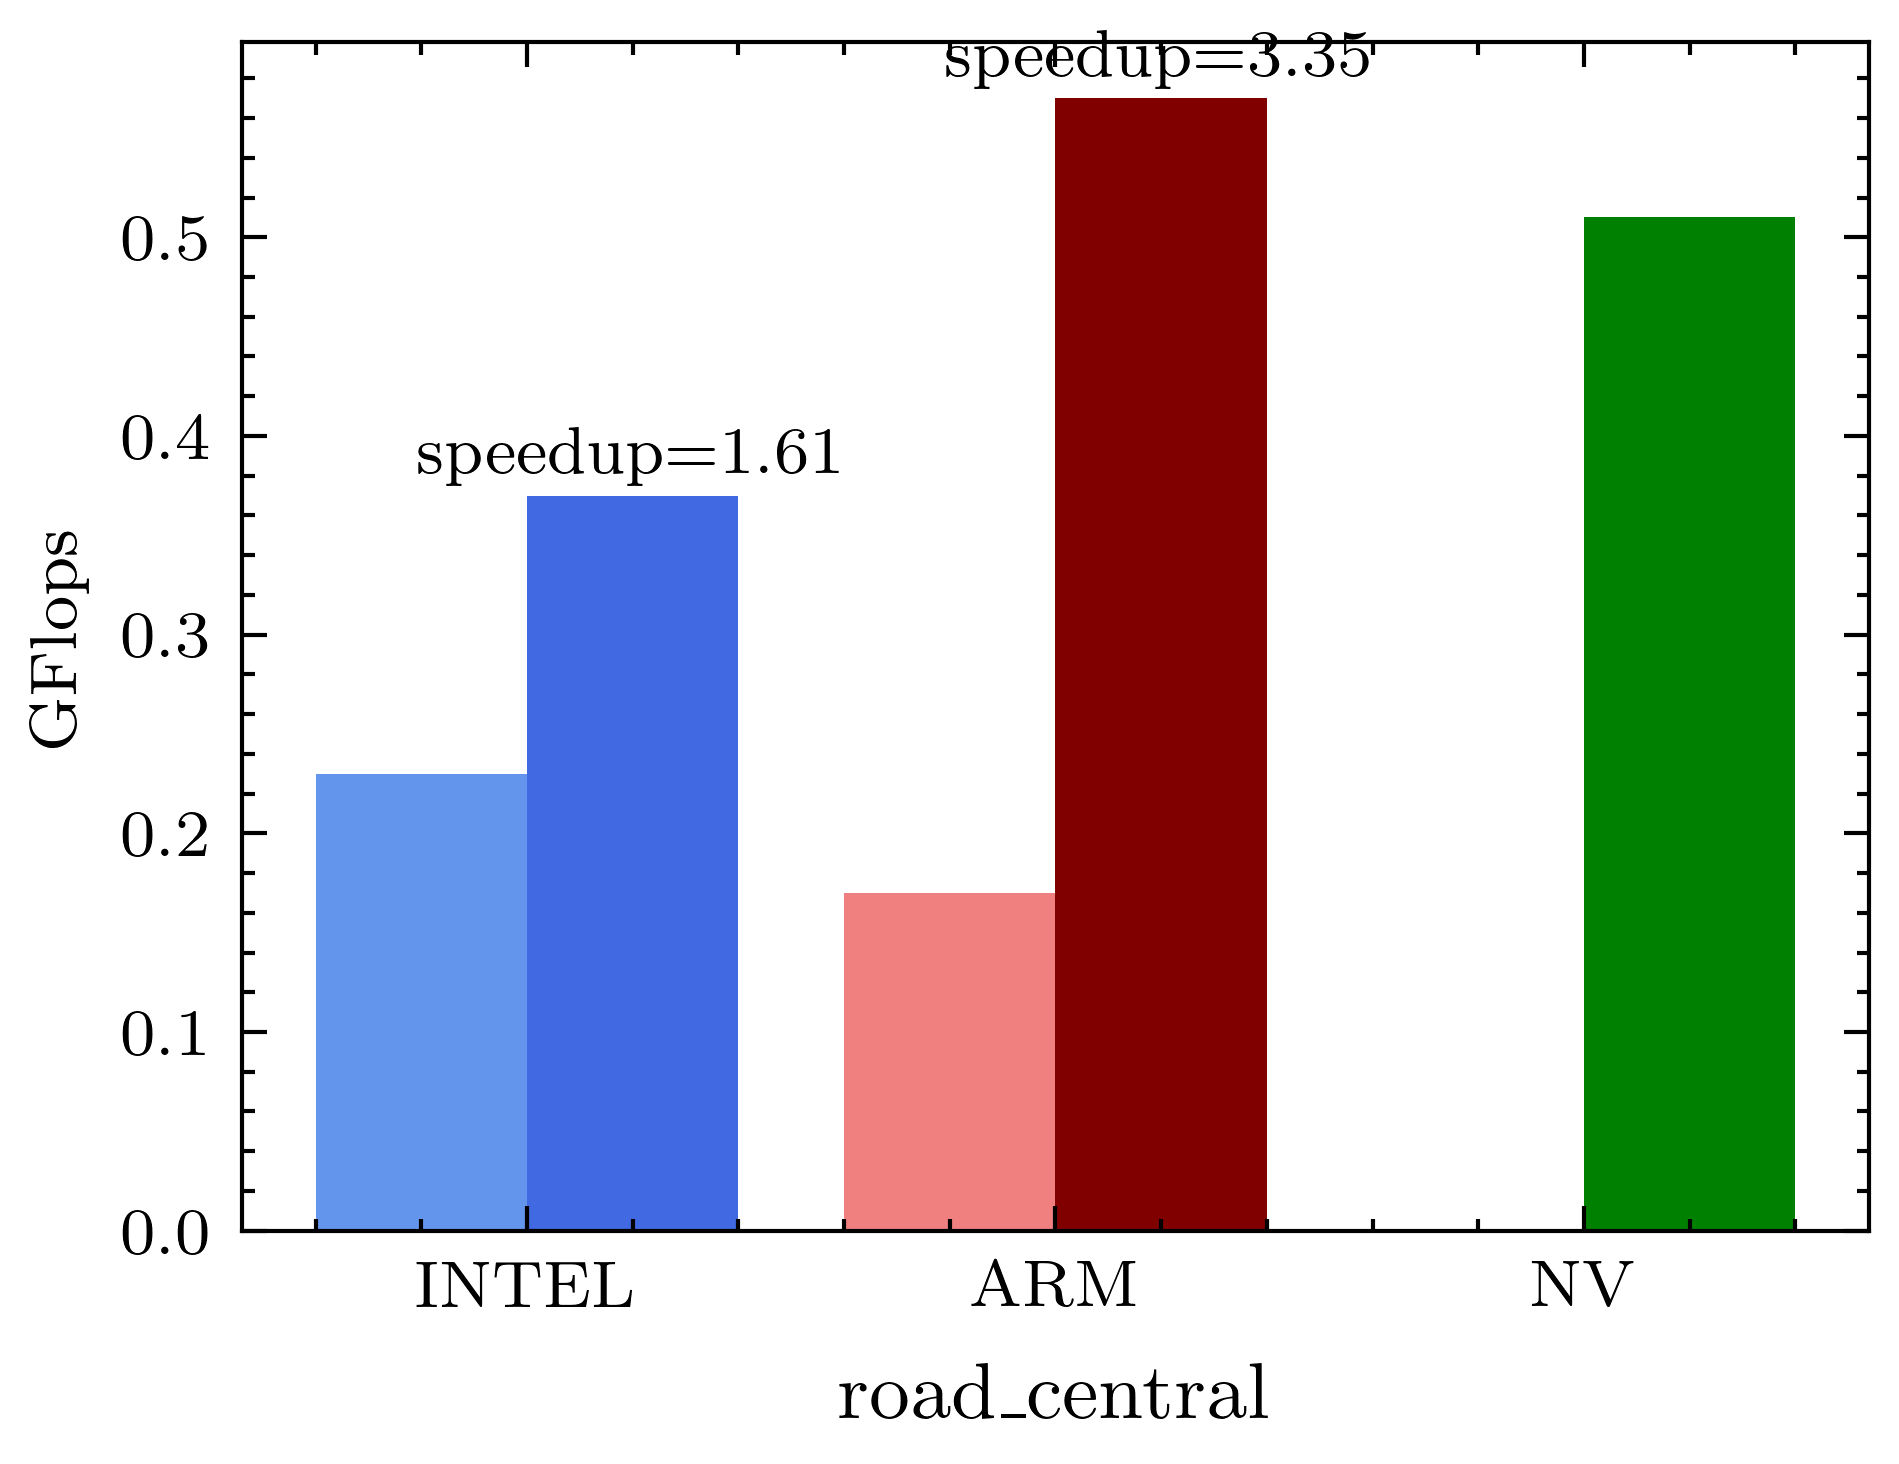
\includegraphics[width=6.5cm]{result1.png}
    }
    \quad
    \subfigure{
    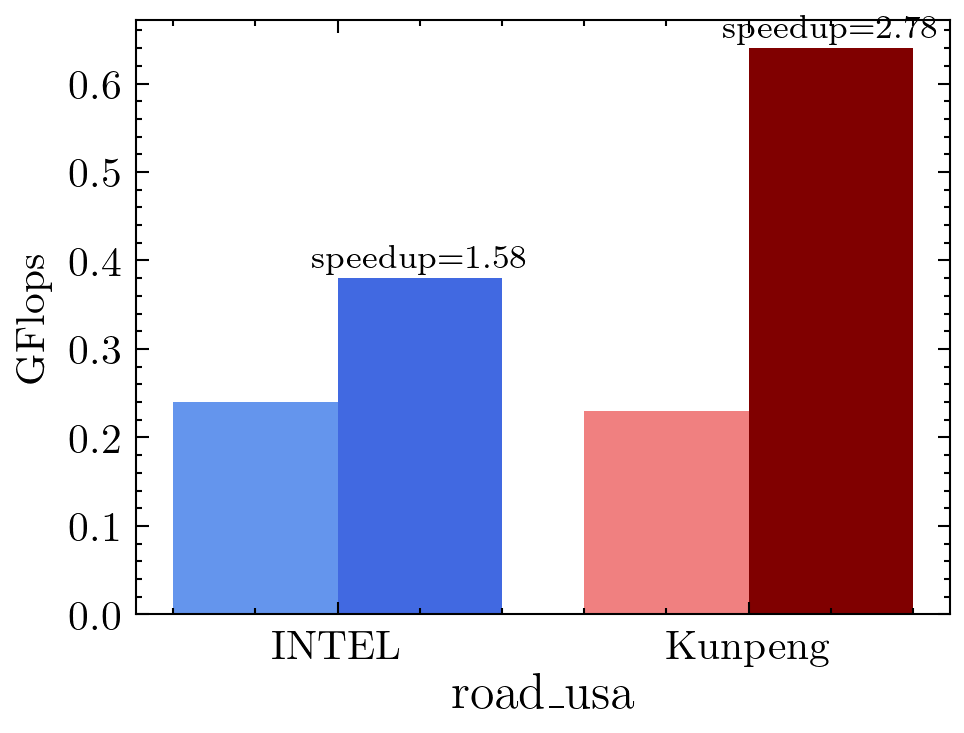
\includegraphics[width=6.5cm]{result2.png}
    }
    \quad
    \subfigure{
    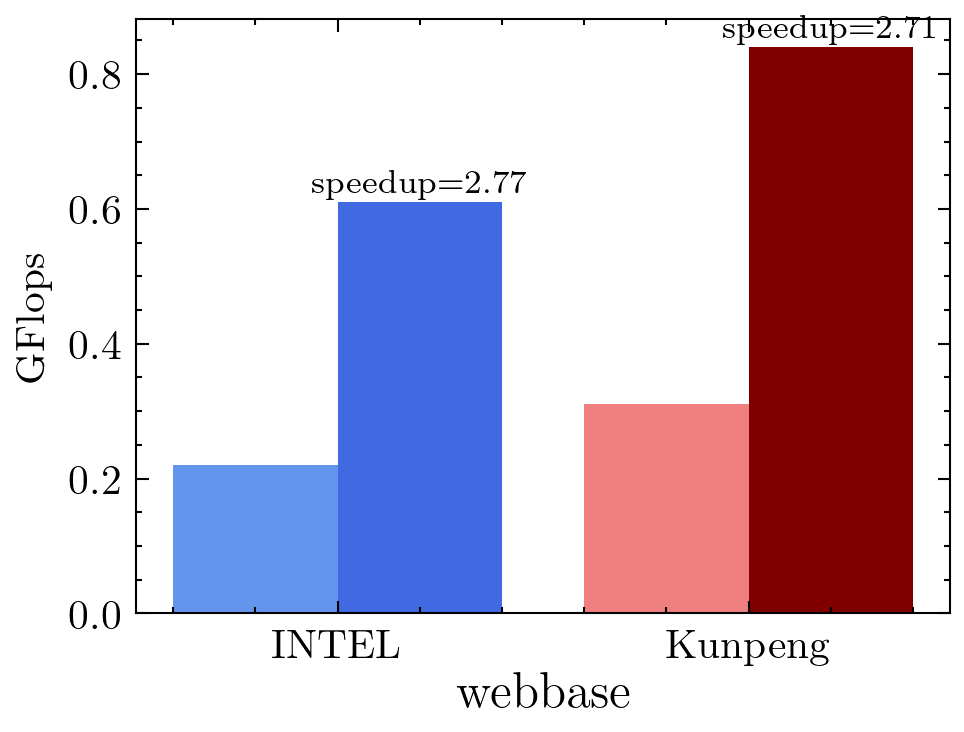
\includegraphics[width=6.5cm]{result3.png}
    }
    \quad
    \subfigure{
    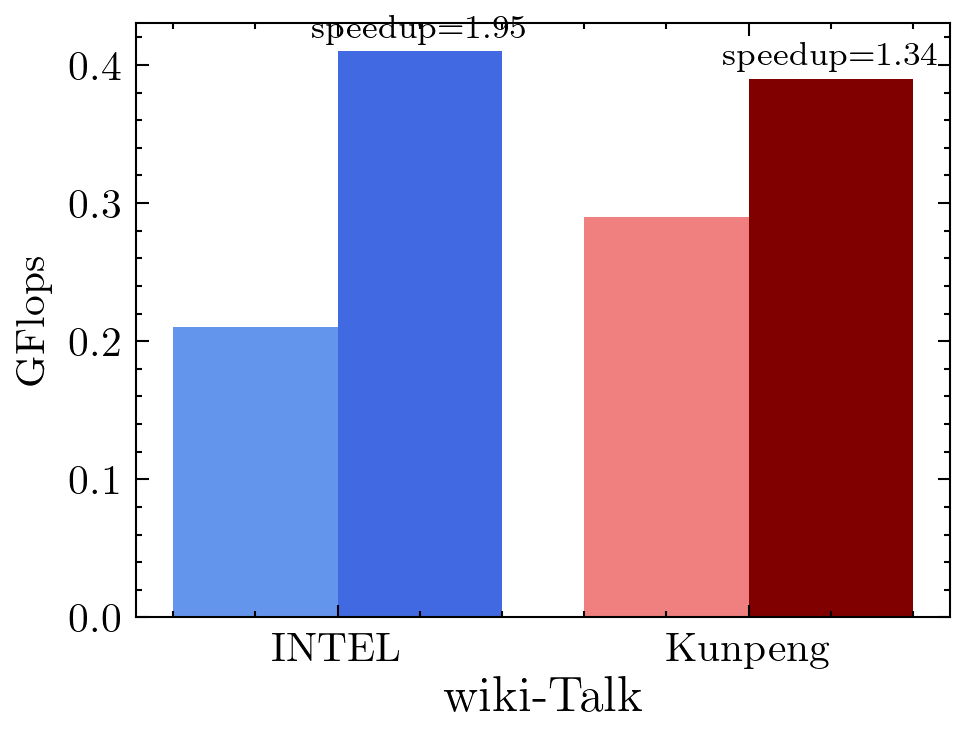
\includegraphics[width=6.5cm]{result4.png}
    }
    \quad
    \subfigure{
    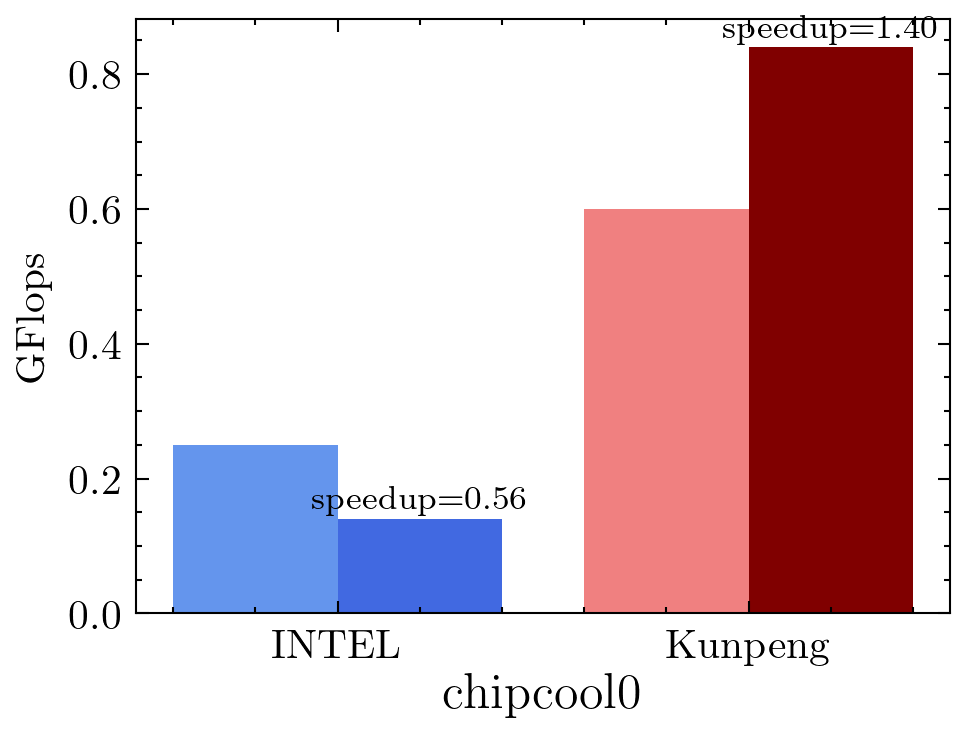
\includegraphics[width=6.5cm]{result5.png}
    }
    \caption{对比不同平台SpTRSV算法的结果示意图}
    \label{SpTRSVMulti-paltform}
\end{figure}

\begin{table}[htbp]
    \resizebox{\textwidth}{!}{%
    \begin{tabular}{|l|r|r|r|r|}
    \hline
    矩阵名称         & 预处理时间 & 计算消耗时间 & 总时间(ms) & 预处理时间占总时间的比例 \\ \hline
    nlpkkt160    & 18.70 & 68.68  & 87.38   & 21.4\%       \\
    road\_central & 20.85 & 87.76  & 108.61  & 19.1\%       \\
    road\_usa     & 42.08 & 141.9  & 77      & 22.8\%       \\
    webbase-1M   & 1.30  & 4.29   & 514     & 23.2\%       \\
    wiki-Talk    & 3.82  & 13.91  & 522     & 21.5\%       \\
    chipcool0    & 0.12  & 0.24   & 534     & 33.3%       
    \end{tabular}%
    }
    \caption{算法耗时分解表}
    \label{算法耗时分解表}
\end{table}

如表\ref{算法耗时分解表}所示,算法在预处理阶段主要进行in\_degree的计算,已经通过任务划分的方式进行负载均衡的处理。预处理时间占总时间的20\%左右,且相对稳定。而且,相比于J.Park\cite{park2014sparsifying}基于level-sets的算法\ref{任务耗时分解图},我的算法在预处理阶的时间消耗很少,例如对于矩阵nlpkkt,基于level-sets的算法需要484.07ms的时间,而我的算法只需要18.70ms的预处理时间,以及68.68ms的计算时间。

\section{测试负载均衡的影响}

对于一些任务任务之间,负载相对均衡的矩阵如nlpkkt160,road\_central和road\_usa,负载均衡优化的开启和关闭,并没有很大的影响,相反对于webbase和chipcool,这两个矩阵之间存在这负载不均衡的想象,所以启用负载均衡起到了优化的作用。由于负载均衡所消耗的时间相对较小,所以并没有对整体的计算时间产生很大的影响。

\begin{figure}[htbp]
    \centering
    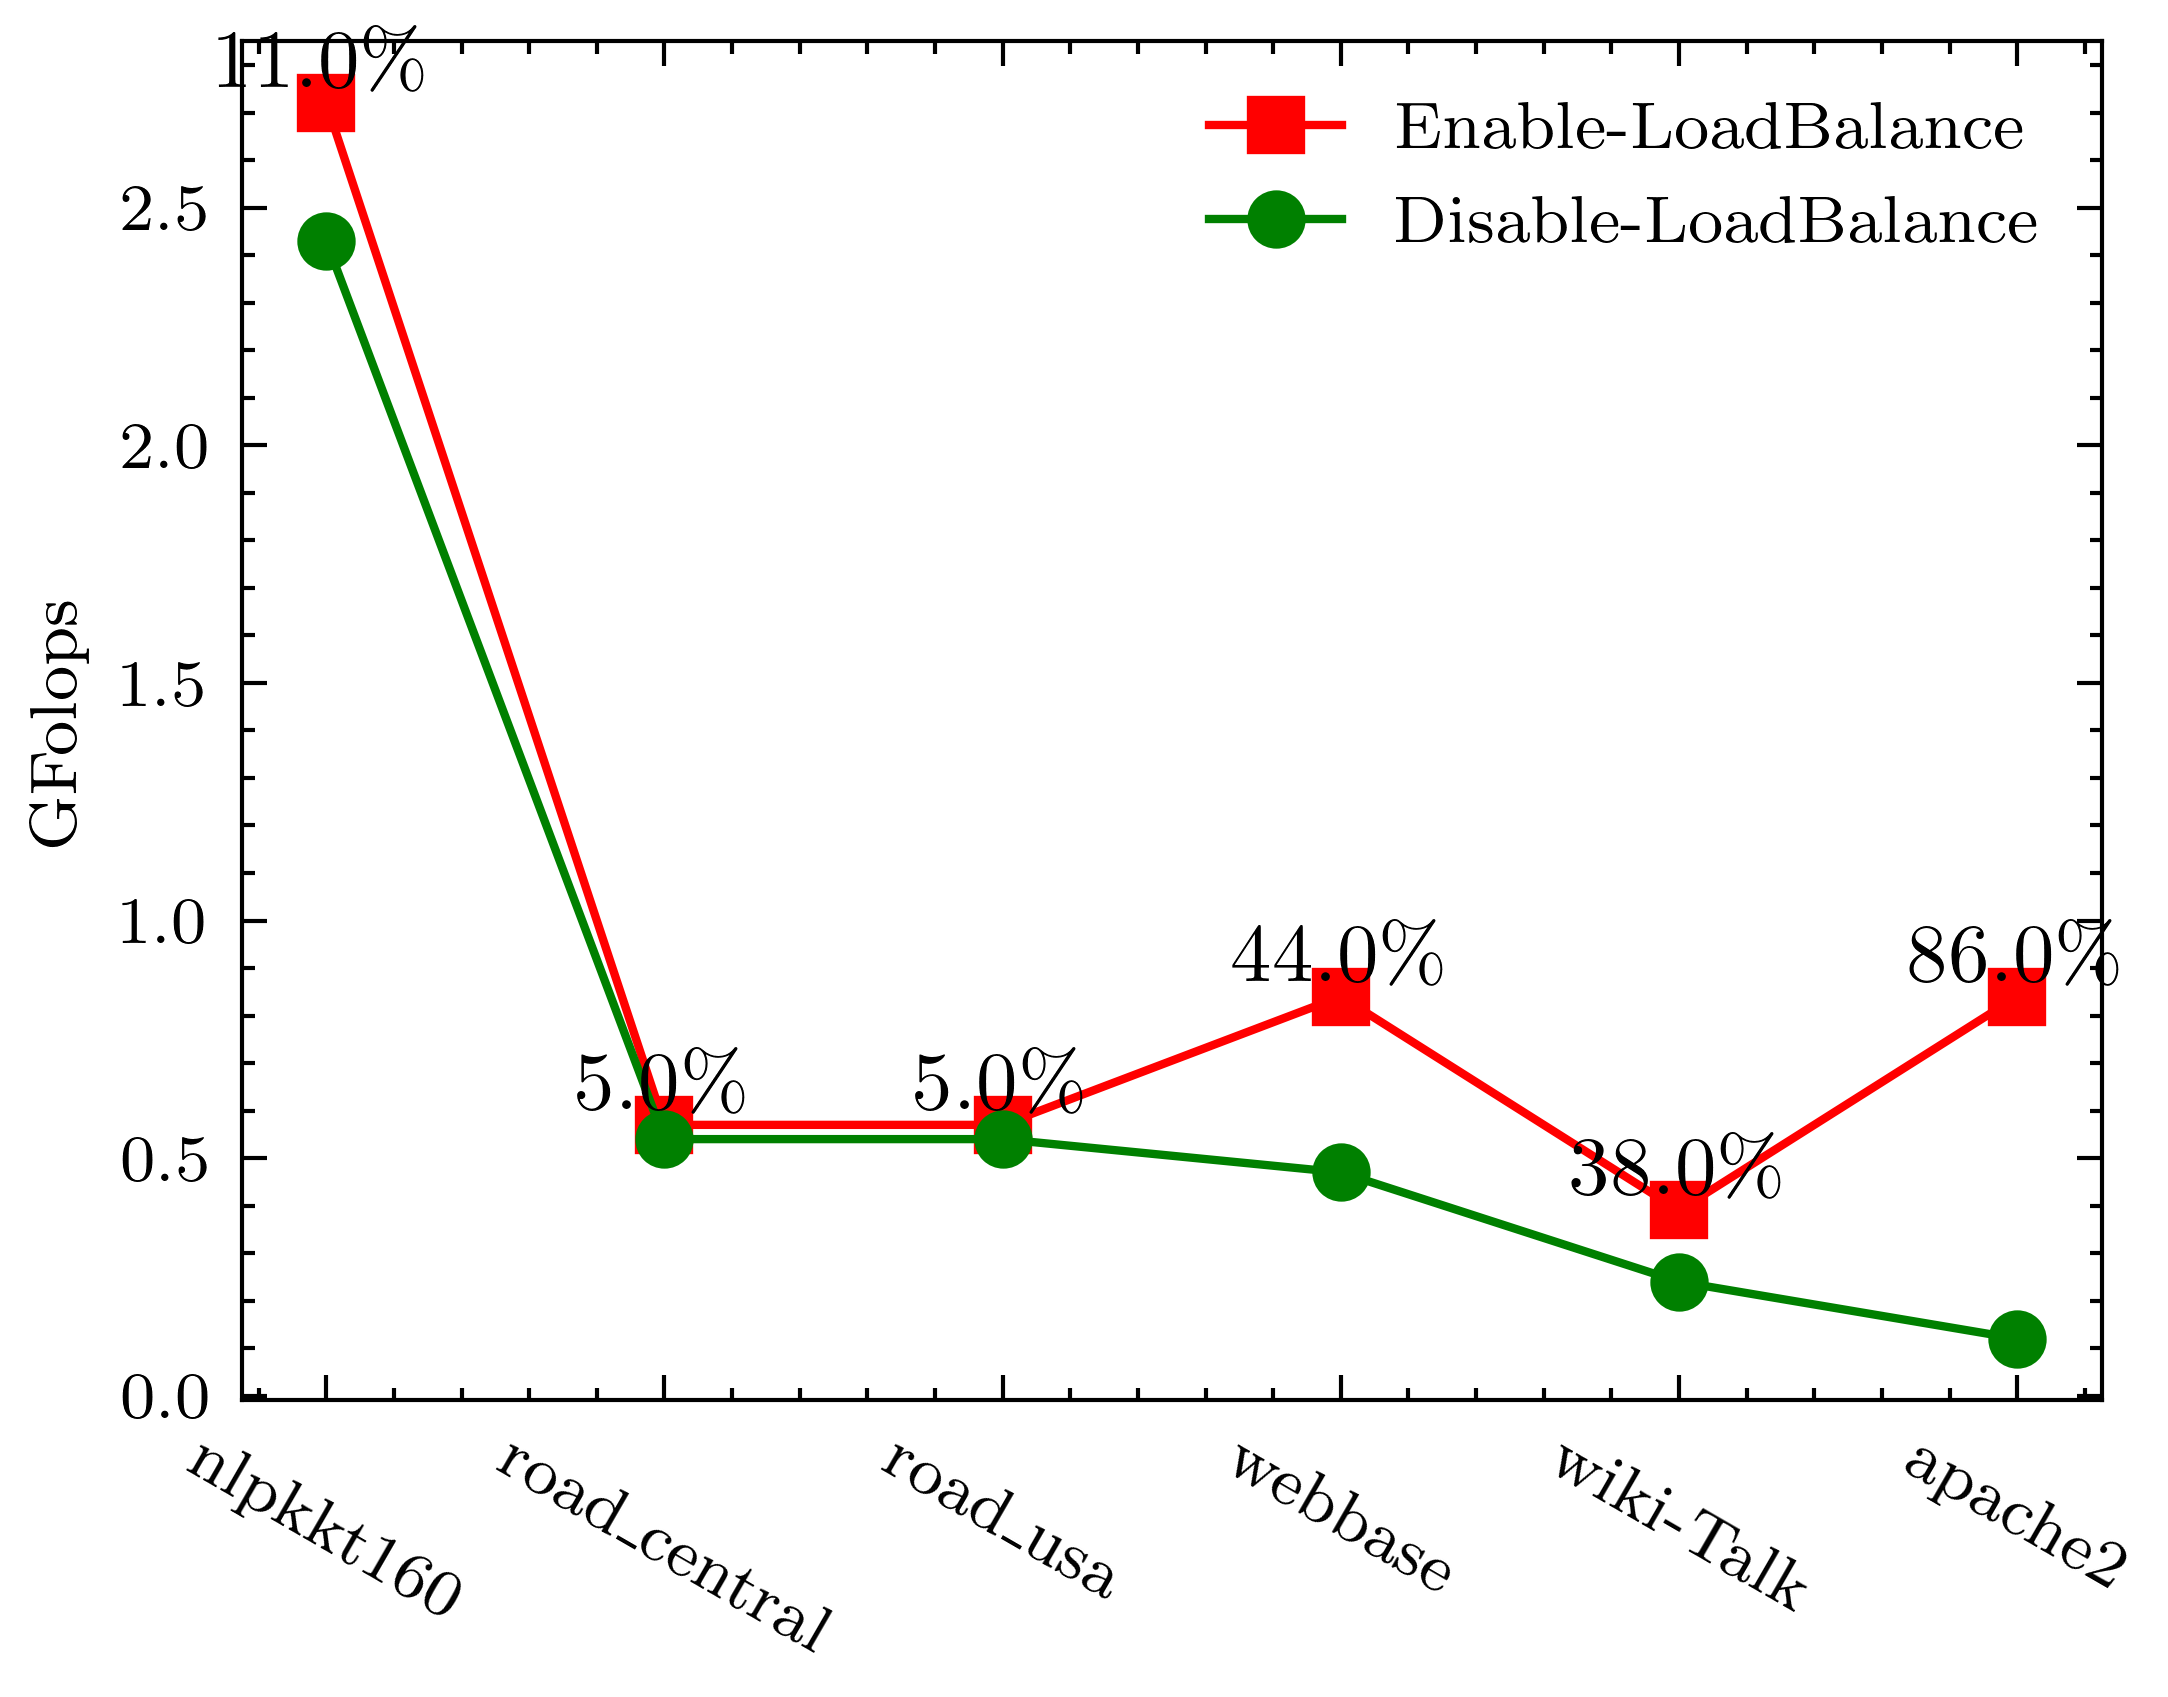
\includegraphics[width=0.7\textwidth]{lbtest.png}
    \caption{测试负载均衡对SpTRSV算法性能的影响}
    \label{测试负载均衡对SpTRSV算法性能的影响}
\end{figure}

\section{使用CPU松弛技术对性能的提升}

\begin{figure}[htbp]
    \centering
    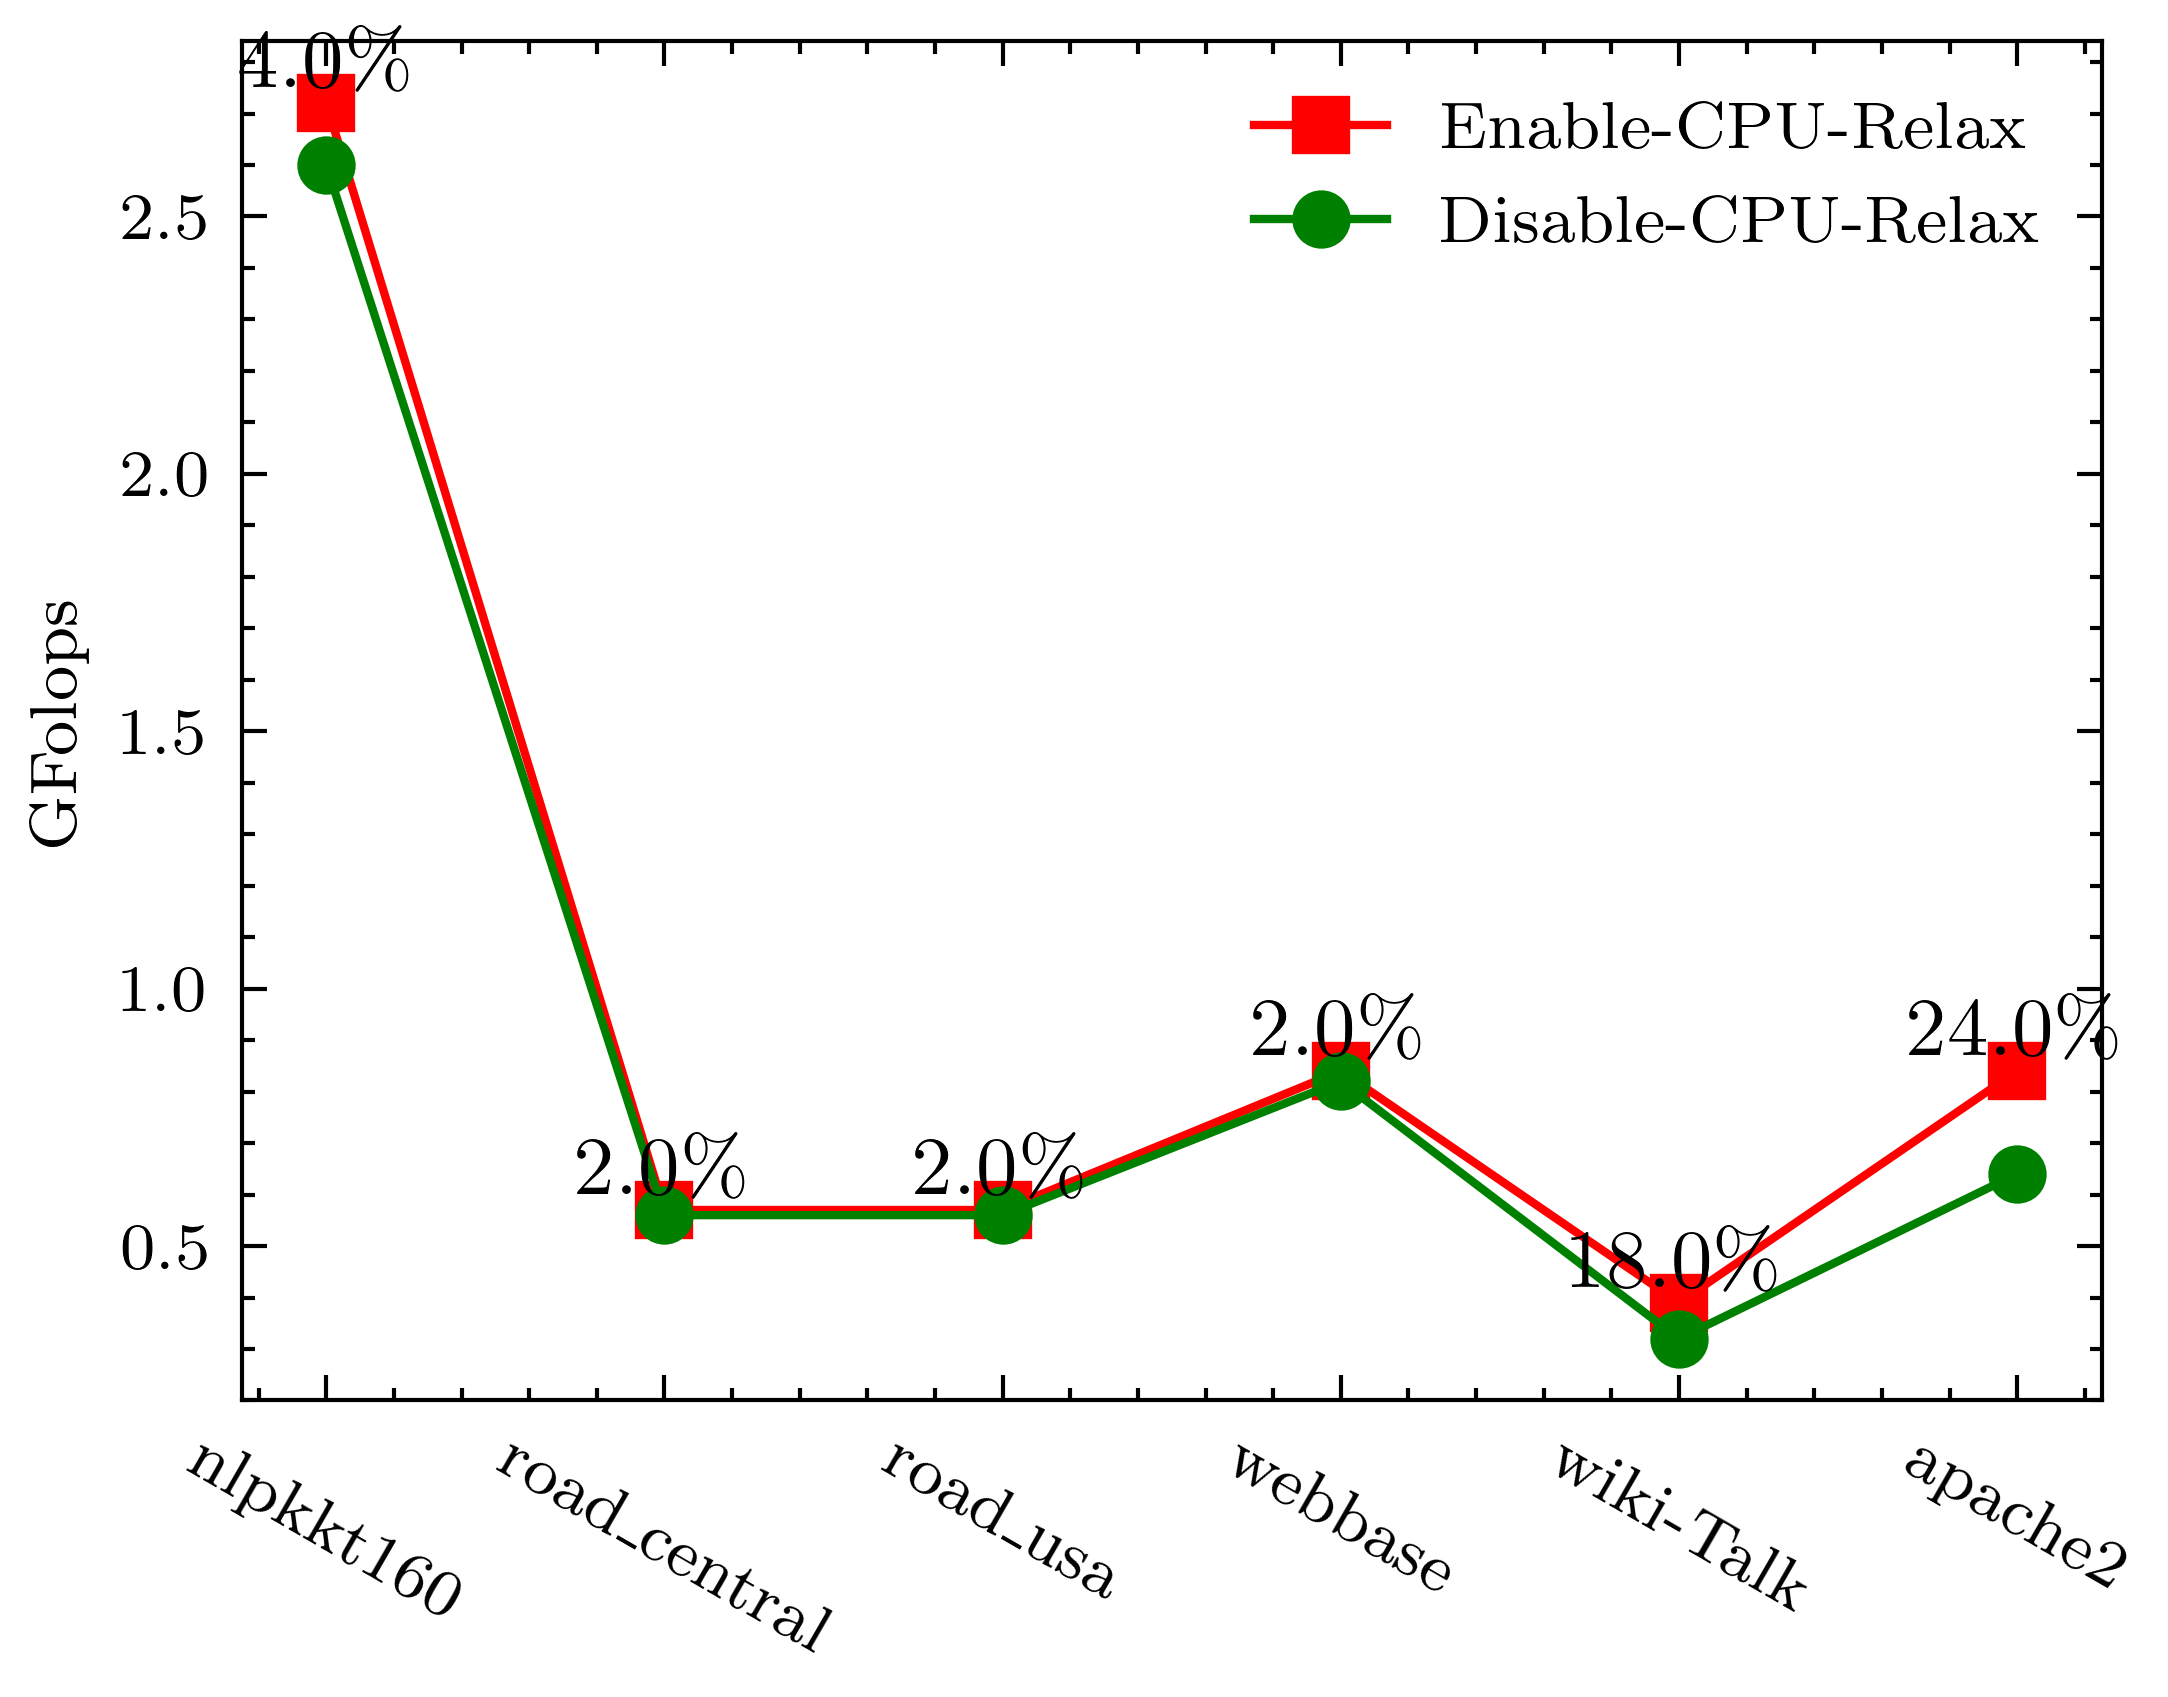
\includegraphics[width=0.7\textwidth]{cpuRelaxTest.png}
    \caption{测试CPU松弛技术对性能的影响}
    \label{测试CPU松弛技术对性能的影响}
\end{figure}
CPU松弛技术对性能地提升相对较低,对于一些任务间依赖相对比较严重的稀疏矩阵有一定的性能提升。

\section{使用ARMv8原子指令对性能的提升}

\begin{figure}[htbp]
    \centering
    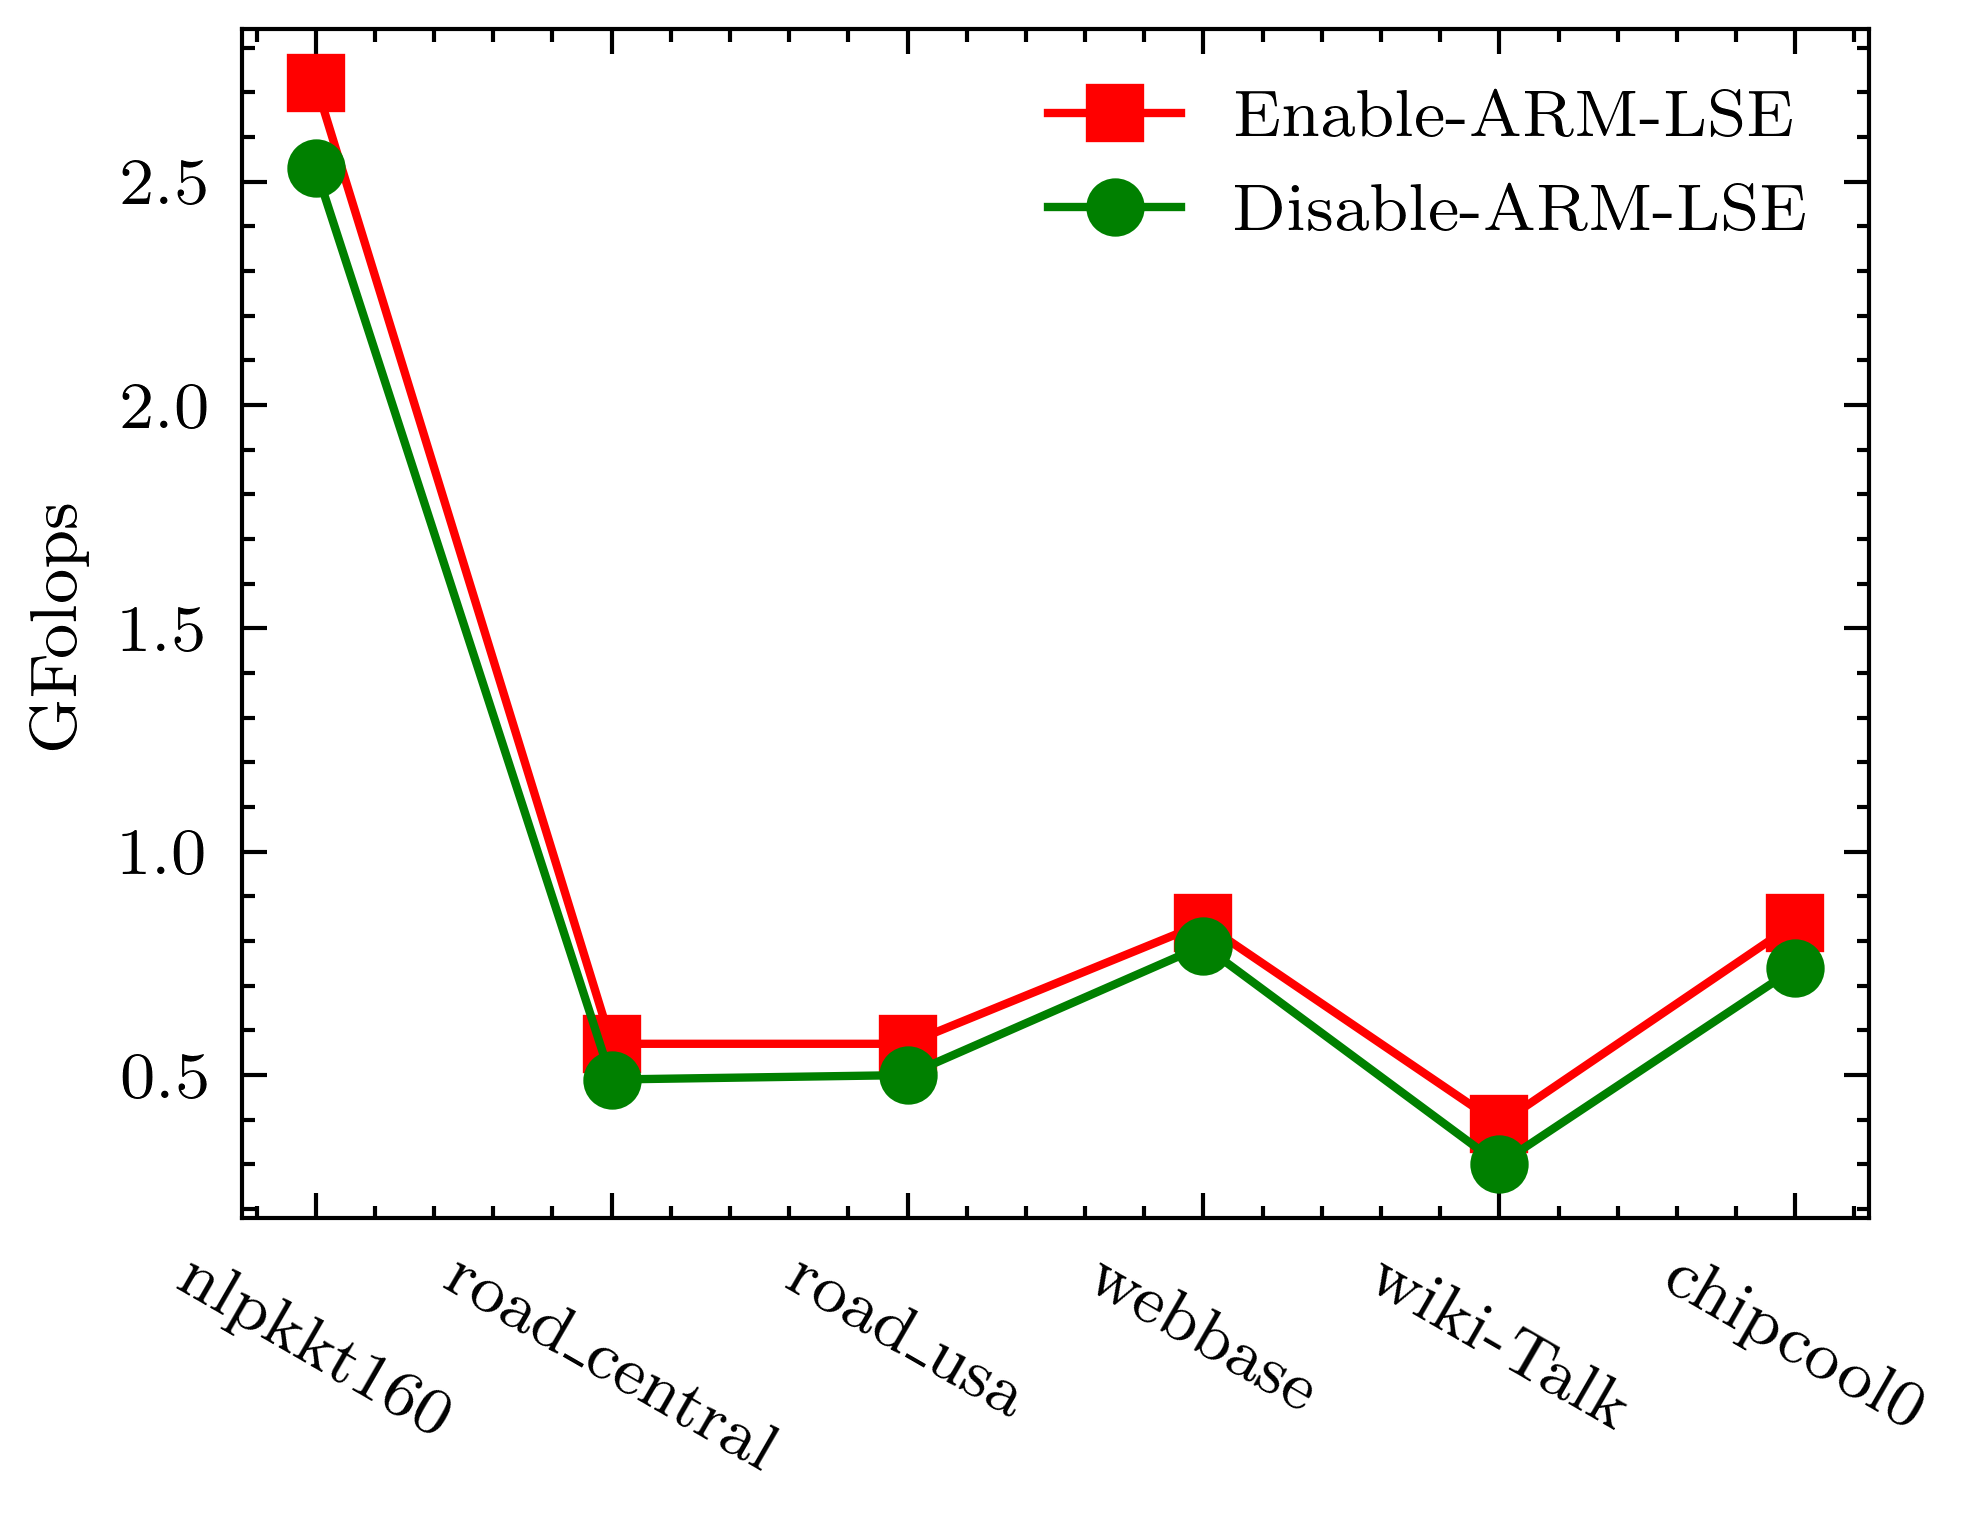
\includegraphics[width=0.7\textwidth]{ARMLSETEST.png}
    \caption{测试ARMv8原子指令对性能的影响}
    \label{测试ARMv8原子指令对性能的影响}
\end{figure}

在使用了ARMv8原子指令之后,性能相比于ARM传统的原子指令,性能有所提升。

% \section{NUMA架构的性能对比测试}

% 同时也应该包含通过NUMA架构对预处理操作的优化。

% TODO这里是一个折线图,应该有五条曲线,分别为串行的情况,以及那四种NUMA策略。


\section{本章总结}

在本章中,我展示了本算法的性能,并与其他平台现有的SpTRSV算法性能进行了对比,见图\ref{MatrixSuite}。同时我也进一步展示算法的在预处理阶段和计算阶段分别占用的时间,见表\ref{算法耗时分解表},相比于基于level-sets的算法,本算法的预处理时间大大减少。最后我也展示了我所使用的三个优化技巧对性能的提升。




\endinput